\documentclass[12pt]{article}
\usepackage{times} 			% use Times New Roman font

\usepackage[margin=1in]{geometry}   % sets 1 inch margins on all sides
\usepackage{hyperref}               % for URL formatting
\usepackage[pdftex]{graphicx}       % So includegraphics will work
\setlength{\parskip}{1em}           % skip 1em between paragraphs
\usepackage{indentfirst}            % indent the first line of each paragraph
\usepackage{datetime}
\usepackage[small, bf]{caption}
\usepackage{listings}               % for code listings
\usepackage{xcolor}                 % for styling code
\usepackage{multirow}

%New colors defined below
\definecolor{backcolour}{RGB}{246, 246, 246}   % 0xF6, 0xF6, 0xF6
\definecolor{codegreen}{RGB}{16, 124, 2}       % 0x10, 0x7C, 0x02
\definecolor{codepurple}{RGB}{170, 0, 217}     % 0xAA, 0x00, 0xD9
\definecolor{codered}{RGB}{154, 0, 18}         % 0x9A, 0x00, 0x12

%Code listing style named "gcolabstyle" - matches Google Colab
\lstdefinestyle{gcolabstyle}{
  basicstyle=\ttfamily\small,
  backgroundcolor=\color{backcolour},   
  commentstyle=\itshape\color{codegreen},
  keywordstyle=\color{codepurple},
  stringstyle=\color{codered},
  numberstyle=\ttfamily\footnotesize\color{darkgray}, 
  breakatwhitespace=false,         
  breaklines=true,                 
  captionpos=b,                    
  keepspaces=true,                 
  numbers=left,                    
  numbersep=5pt,                  
  showspaces=false,                
  showstringspaces=false,
  showtabs=false,                  
  tabsize=2
}

\lstset{style=gcolabstyle}      %set gcolabstyle code listing

% to make long URIs break nicely
\makeatletter
\g@addto@macro{\UrlBreaks}{\UrlOrds}
\makeatother

% for fancy page headings
\usepackage{fancyhdr}
\setlength{\headheight}{13.6pt} % to remove fancyhdr warning
\pagestyle{fancy}
\fancyhf{}
\rhead{\small \thepage}
\lhead{\small HW3, Bartels}  % EDIT THIS, REPLACE # with HW number
\chead{\small CS 432, Fall 2020} 

%-------------------------------------------------------------------------
\begin{document}

\begin{centering}
{\large\textbf{HW3 - Ranking Webpages}}\\ % EDIT THIS
                                % REPLACE # with HW num and ADD title
Logan Bartels\\                     % EDIT THIS
October 18, 2020\\                      % EDIT THIS
\end{centering}

%-------------------------------------------------------------------------

% The * after \section just says to not number the sections
\section*{Note}
\textbf{All scripts were tested by using ``testLinks.txt'' as the staring input file instead of ``uniqueTwitterLinks.txt''.}

\section*{Q1}

\subsection*{Answer}

\lstinputlisting[language=sh, caption=Bash script used to parse unique list of Twitter links and download their content to an output file., label=lst:download]{readFile.sh}

\lstinputlisting[language=sh, caption=Bash script used to parse the list of hashed file names to open them and remove html markup., label=lst:process]{processFiles.sh}


\subsection*{Discussion}
The script in listing \ref{lst:download} parses the unique list of links line-by-line.  It then hashes the URI into an appropriate file name and stores it in a variable, ``fileName''.  Curl is then used on the link to download the content and direct the output to the value in the ``fileName'' variable with ``.html'' appended to the end of the file name.  The URI is appended at the end of the hashed file to keep track of the original URIs.  The appended URI in the hashed file can be easily viewed in a text editor.  The hashed file name is then added to a file that lists the hashed file names, ``fileNames.txt''.

The script in listing \ref{lst:process} reads the list of hashed file names line-by-line.  For each line, JusText is ran on the file listed in the line to remove html markup.  The output is directed to the same filename with ``processed'' added as a prefix to keep track of files put through JusText.  The processed file name is then added to a file that lists the processed file names, ``processedFileNames.txt''.


\section*{Q2}

\subsection*{Answer}

\lstinputlisting[language=sh, caption=Bash script used search for the term ``Trump'' in each processed html document; output directed to trumpFiles.txt at the command line., label=lst:search]{search.sh}

\lstinputlisting[caption=Output of files containing the term ``Trump''; each file is preceded by the number of times ``Trump'' appears in the file., label=lst:trumpFiles]{trumpFiles.txt}

\lstinputlisting[caption=List of files chosen to compute TF-IDF values for., label=lst:usedFiles]{trumpFilesUsed.txt}

List of URIs referenced in table \ref{tbl:TFIDF}.

\begin{enumerate}

    \item \url{ https://finance.yahoo.com/news/win-presidency-001318552.html?soc_src=social-sh&soc_trk=tw&tsrc=twtr }
    \item \url{ https://apnews.com/article/election-2020-virus-outbreak-seniors-florida-michael-pence-b8bbfd3a87dc290a84b9ed9915a4cf63 }
    \item \url{ https://abcnews.go.com/Politics/candace-owens-blexit-group-pays-attendees-travel-trumps/story?id=73531036 }
    \item \url{ https://apnews.com/5e833a62e9492f6a66624b7920cc846a }
    \item \url{ https://apnews.com/article/election-2020-joe-biden-donald-trump-pennsylvania-lawsuits-15e9dfeede4ddee5086611f0dd7b63a0 }
    \item \url{ https://apnews.com/article/virus-outbreak-donald-trump-a6c145029afb7a28bd739969387813e8 }
    \item \url{ https://apnews.com/ed5453fa2078982dba31919b8c1e274f }
    \item \url{ https://dailycaller.com/2020/10/09/commission-presidential-debates-board-members-anti-donald-trump/ }
    \item \url{ https://hillreporter.com/moodys-analytics-a-joe-biden-presidency-would-create-7-million-more-jobs-than-trumps-81808 }
    \item \url{ https://news.yahoo.com/judge-battleground-state-tosses-trump-220917951.html?soc_src=hl-viewer&soc_trk=tw }
    
\end{enumerate}

\begin{table}[h]

\centering
\caption{TF-IDF values for ``Trump'' using Bing as the corpus}
\label{tbl:TFIDF}
\begin{tabular}{|l|l|l||l|}
\hline
\textbf{TF-IDF} & \textbf{TF} & \textbf{IDF} & \textbf{URI Number} \\ \hline
0.2 & 0.026 & 7 & 1 \\ \hline
0.1 & 0.020 & 7 & 8 \\ \hline
0.1 & 0.017 & 7 & 10 \\ \hline
0.1 & 0.016 & 7 & 5 \\ \hline
0.1 & 0.015 & 7 & 7 \\ \hline
0.08 & 0.012 & 7 & 2 \\ \hline
0.08 & 0.012 & 7 & 3 \\ \hline
0.08 & 0.012 & 7 & 4 \\ \hline
0.08 & 0.012 & 7 & 9 \\ \hline
0.07 & 0.01 & 7 & 6 \\ \hline


\end{tabular}
\end{table}

\begin{figure}[h]

    \centering
    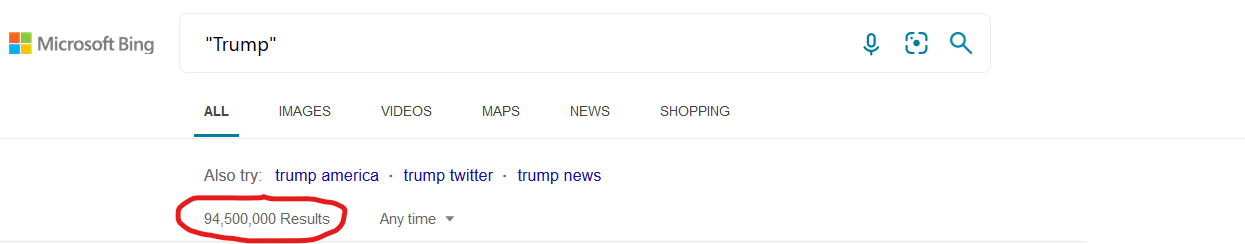
\includegraphics[trim=0 0 280 0]{trumpBingResults.png}
    \caption{Results from the query ``Trump'' using Bing}
    \label{fig:query_results}
    
\end{figure}

\subsection*{Discussion}
The potential candidates for computing TF-IDF values were determined by using the script listed in listing \ref{lst:search}.  The script in listing \ref{lst:search} reads the list of processed files created by listing \ref{lst:process} line-by-line.  For each line, the script counts how many times ``Trump'' appears in the file listed.  The value is stored in the ``count'' variable.  A check is performed to see if count=0.  If it does, then the iteration is skipped.  If it does not, then ``grep -c'' is performed again, as well as ``grep-l''.  This format shows how many times the term ``Trump'' appears in the file, and the file name.  The output was directed to ``trumpFiles.txt'' (shown in listing \ref{lst:trumpFiles}) when the shell script was run at the command line.  

The list of files used to compute TF-IDF values are shown in listing \ref{lst:usedFiles}.  The filenames are only listed to the point of being able to complete a successful search in File Explorer on Windows, or being able to successfully use tab-completion in bash.

Term frequency was calculated by using the ``grep -c'' command, and dividing the returned number by the value returned by the ``wc -w'' command used on the processed html document.  The term frequency value in the table for each URI is rounded to two significant figures, with the exception of URI number six, because the numerator in its TF calculation only had one significant figure.  The IDF  was determined by dividing ten billion by ninety-four-million-five-hundred-thousand (shown in Figure \ref{fig:query_results}).  Since ten billion only has one significant figure, the final IDF answer in the table was rounded to seven.  The TF-IDF values for each URI were calculated by multiplying the TF and IDF values in the table for each URI.  The TF-IDF values for each URI in the table are rounded to one significant figure, each.  All calculations were done manually with a TI-84 calculator.


\section*{Q3}

\subsection*{Answer}

\begin{table}[h]

\centering
\caption{Page Rank Values}
\label{tbl:PageRank}
\begin{tabular}{|c|c|}
\hline
\textbf{Page Rank} & \textbf{URI Number} \\ \hline
8 & 10 \\ \hline
7 & 1 \\ \hline
7 & 8 \\ \hline
7 & 5 \\ \hline
7 & 7 \\ \hline
7 & 2 \\ \hline
7 & 3 \\ \hline
7 & 4 \\ \hline
7 & 6 \\ \hline
6 & 9 \\ \hline


\end{tabular}
\end{table}

\subsection*{Discussion}
Page ranks were determined by \url{https://dnschecker.org/pagerank.php}  Given that my ten URIs point to news websites, it's not surprising that their page ranks are in the 6-8 range.  Five out of the ten URIs changed places.  Notably, URI 10 moved up 2 rows, URI 1 moved down 1 row, URI 8 moved down 1 row, and URIs 6 and 9 switched places.

\section*{References}

\begin{itemize}
    \item { JusText GitHub, \url{ https://github.com/miso-belica/jusText }}
    \item { module 'cgi' has no attribute 'escape', \url{ https://github.com/trustedsec/social-engineer-toolkit/issues/721 }}
    \item { How to Use the grep Command on Linux, \url{ https://www.howtogeek.com/496056/how-to-use-the-grep-command-on-linux/ }}
    \item { How to Create/Write a Simple/Sample Linux Shell/Bash Script, \url{ https://www.instructables.com/How-to-Write-a-Linux-Shell-Script/ }}
    \item { HowTo: Bash For While Loop Through File Contents Script, \url{https://www.cyberciti.biz/faq/linux-unix-appleosx-bsd-bash-loop-through-file-contents/ }}
    \item { Linux/UNIX: Bash Read a File Line By Line, \url{ https://www.cyberciti.biz/faq/unix-howto-read-line-by-line-from-file/ }}
    \item { Bash Beginner Series \#8: Loops in Bash, \url{ https://linuxhandbook.com/bash-loops/ }}
    \item { BASH command output to the variable, \url{ https://linuxhint.com/bash_command_output_variable/ }}
    \item { Bash conditional statement, \url{ https://linuxhint.com/bash_conditional_statement/ }}
    \item { Shebang, \url{https://bash.cyberciti.biz/guide/Shebang }}
    \item { Writing output to files, \url{ https://bash.cyberciti.biz/guide/Writing_output_to_files }}
    \item { Significant Figure Rules for Logarithms, \url{ https://laney.edu/cheli-fossum/wp-content/uploads/sites/210/2018/01/Significant-Figure-Rules-for-logs.pdf }}
    \item { Significant Figures, \url{ https://courses.lumenlearning.com/introchem/chapter/significant-figures/ }}
    \item { Significant figures: Rounding and decimal places, \url{ https://en.wikipedia.org/wiki/Significant_figures#Rounding_and_decimal_places }}
    \item { Pagerank Checker Tool, \url{https://dnschecker.org/pagerank.php }}
    \item { Week-06 Slides, \url{ https://docs.google.com/presentation/d/1rKj7Qdpz0GH0lHl0WYk498-1Lhi0C612j_0hjm4j5X8/edit#slide=id.g32fc6d3dd1_0_4 }}
    
    
\end{itemize}

\end{document}

